% A two-column news report. Heading spanning two columns. Page size roughly A3.
% This code was written during 2008-2015 for Kolkata based Bengali fortnightly Khoborer Kagoj Songbadmanthan.
%============================================
\documentclass{article} 
\usepackage{fontspec} 
\usepackage{xunicode} 
\usepackage{xltxtra} 
\usepackage{multicol} 
\usepackage{ragged2e} 
\usepackage{wrapfig} 
\usepackage{graphicx} 
\usepackage{tikz}
\usetikzlibrary{shadows}
\usetikzlibrary{shapes,snakes}
\usepackage[papersize={11in,18in},top=1in,bottom=1.5in,left=0.5in,right=0.5in]{geometry} 
\usepackage{caption}
\captionsetup{singlelinecheck=false, format=plain, aboveskip=2pt, belowskip=1pt, margin=0pt, labelformat=empty, labelsep=none, justification=justified}
\definecolor{Light}{gray}{0.8}
\definecolor{Dark}{gray}{0.2}
\definecolor{Grey}{gray}{0.65}
%
% These are the fonts and their variations. Baban12 and BabanBold12 fonts are custom made. Font files are provided in the directory. Ubuntu font is available in internet freely. 
\newcommand\EN[1]{	 
\fontsize{#1}{#1}\fontspec{Ubuntu}} 
\newcommand\BN[1]{ % Normal face of the Bengali font
\fontsize{#1}{#1}\fontspec[Script=Bengali]{Baban12}} 
\newcommand\BB[1]{ % Bold face of the Bengali font
\fontsize{#1}{#1}\fontspec[Script=Bengali]{BabanBold12}} 
\newcommand\BI[1]{ % Italic face of the Bengali font
\fontsize{#1}{#1}\fontspec[Script=Bengali, FakeSlant=0.2]{Baban12}} 
\newcommand\BBI[1]{ % Bold italic face of the Bengali font
\fontsize{#1}{#1}\fontspec[Script=Bengali, FakeSlant=0.2]{BabanBold12}} 
%
%
\begin{document}
% 
\begin{minipage}[t]{118mm} % A single news item should be within a minipage environment
\vspace{6mm}
\setlength{\baselineskip}{2pt}
\setlength{\parskip}{0.15ex} 
\setlength{\parindent}{10pt}
\begin{multicols}{2} % Two Column environment starts
[\section*{\Centering\BB{40.22}অনাবৃষ্টির উত্তরবঙ্গে চাষিসমাজ সঙ্কটে\\[3mm]
\setlength{\fboxsep}{0pt}
\setlength{\fboxrule}{0.5pt} \fbox{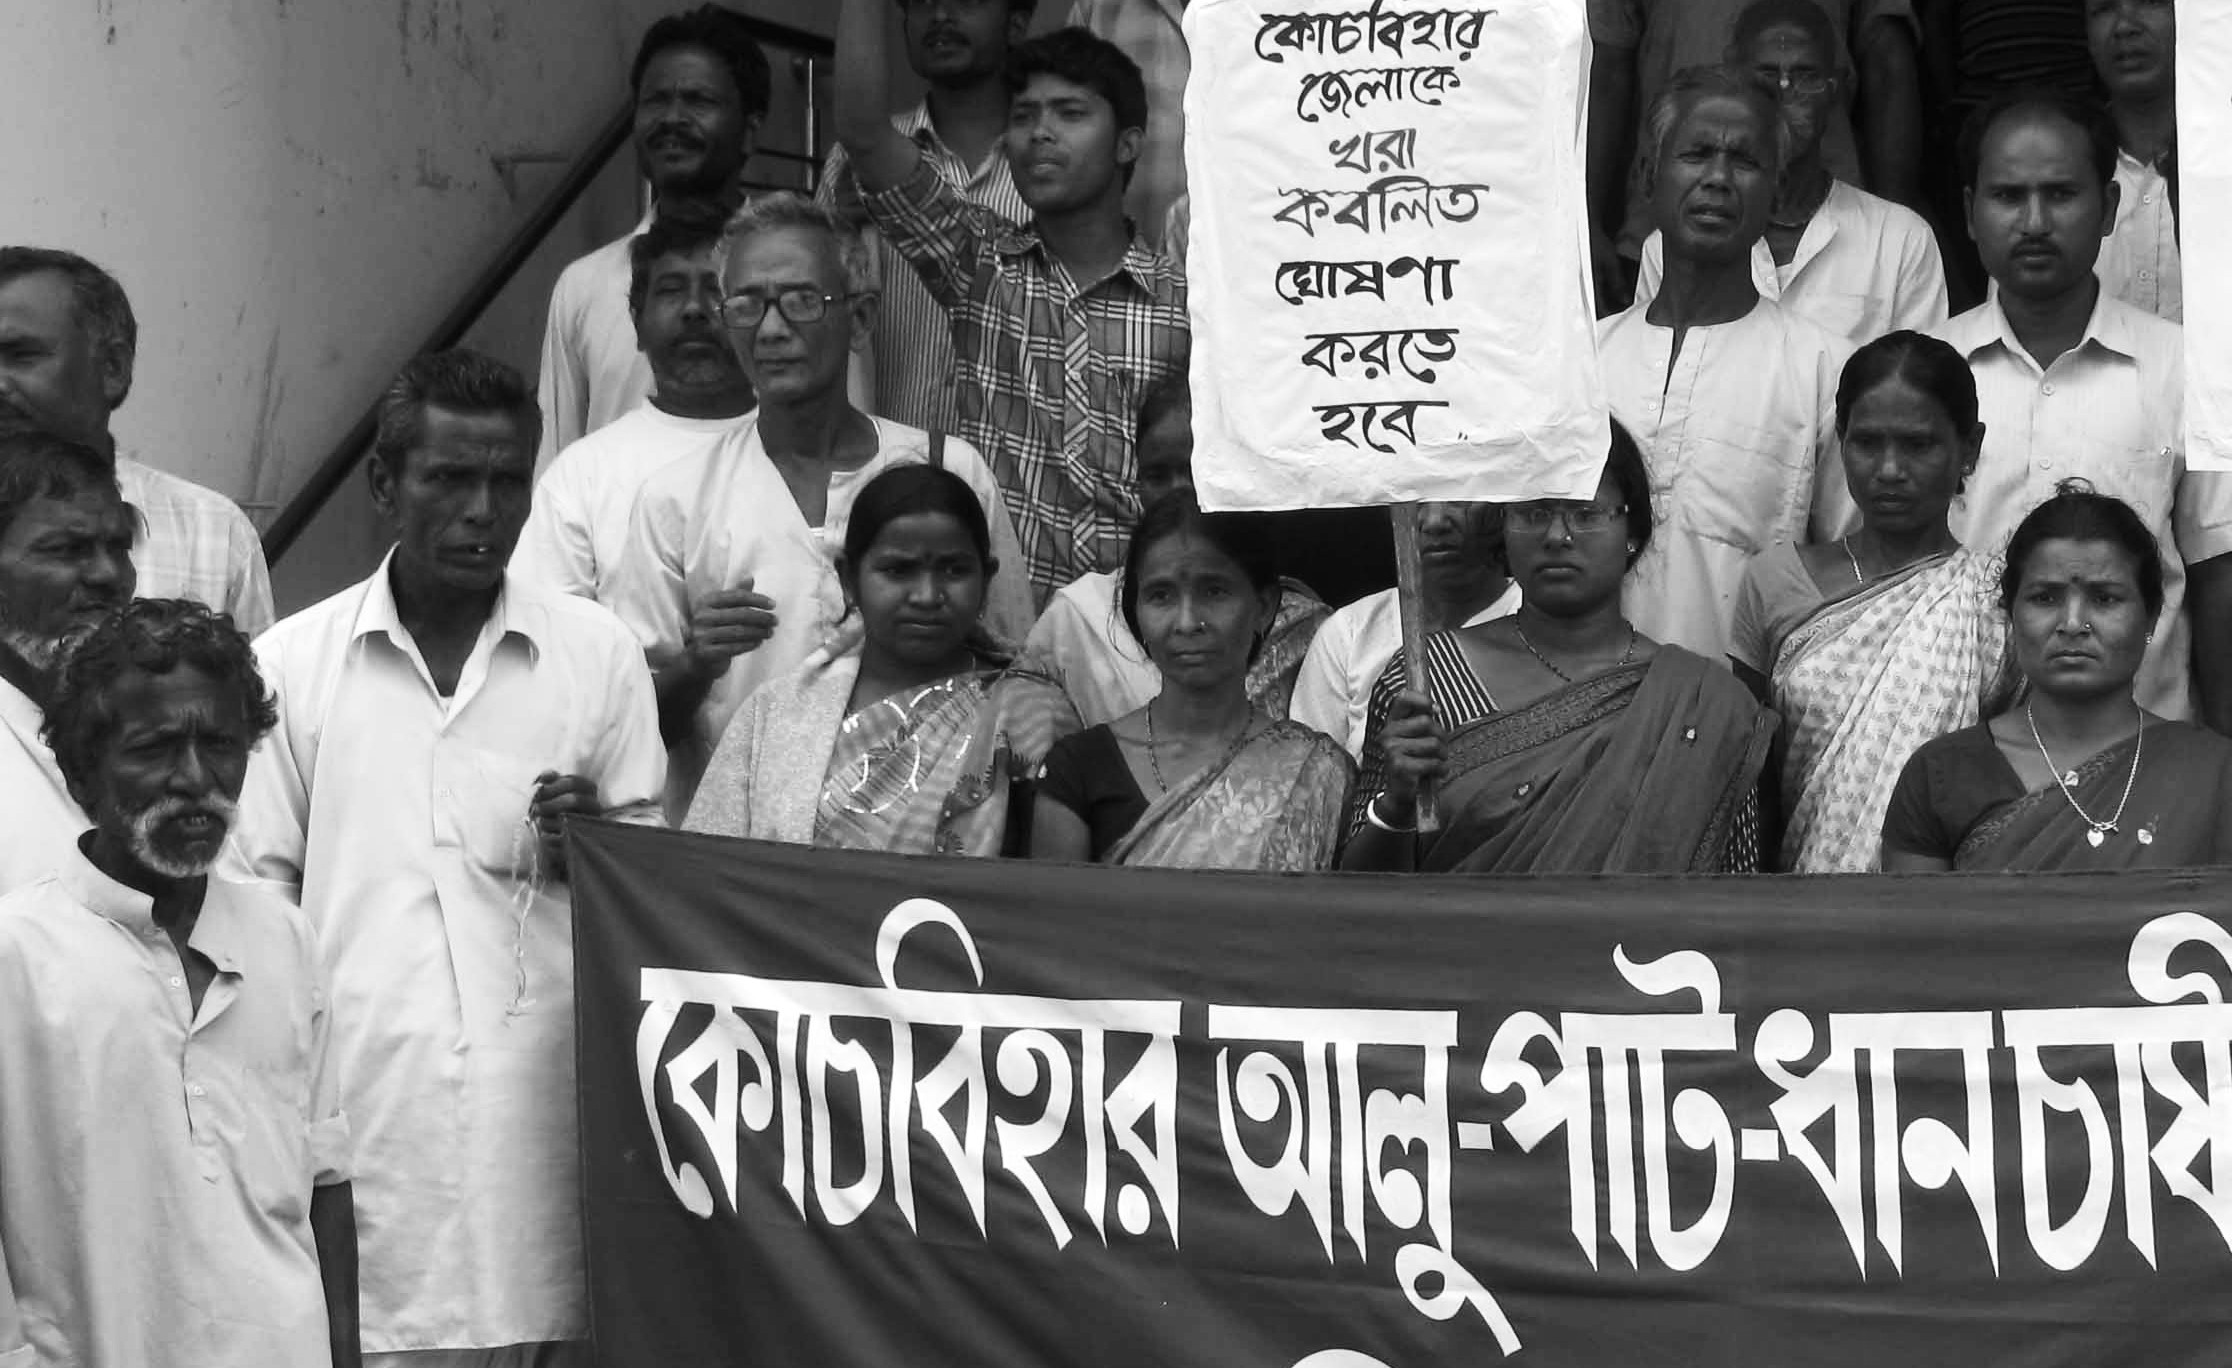
\includegraphics[width=118mm]{krishi.jpg}}
\\[-8mm]
\parbox[t]{118mm}{\Centering\BBI{12.2545}এপ্রিলের শেষ সপ্তাহে কোচবিহার শহরে বিক্ষোভ, ছবি তুলেছেন রামজীবন ভৌমিক। \hspace{1mm}}\\[-11.5mm]
\RaggedLeft
\rule{118mm}{0.5pt}\\[2mm]
}]
% following three lines for adjusting multiple columns. 
\setcounter{columnbadness}{7000}
\setcounter{finalcolumnbadness}{7000}
\tolerance=2000 
%
%
\raisebox{5mm}{\parbox[h]{56mm}{%
%
% Quotation environment declarations
\tikzstyle{mybox} = [draw=black, fill=black!20, thick,
rectangle, rounded corners, inner sep=5pt, inner ysep=10pt]
\tikzstyle{fancytitle} =[fill=black, text=white]
\begin{tikzpicture}% Quotation environment starts here
\node [mybox, right=2pt] at (0.9,-0.1) (box){%
\begin{minipage}{53mm} % A minipage environment for qutation body.
\RaggedRight
\BB{11.06} .\\\hspace{12mm}
সরকার রোদে তেতে যাওয়া কোচবিহার শহরের রাস্তা ঠান্ডা করতে জল ঢালে। সেই জল যদি গ্রাম কোচবিহারের মাঠে ঢালা হত, তাহলে পাটগুলো পুড়ে নষ্ট হত না। -- 
\end{minipage} % minipage environment for qutation body ends here.
};
\node[fancytitle, left=5pt] at (box.north east) {\BBI{11.2545}বিক্ষোভকারী}; % inset at right-top corner of the quotation, place for speaker.
\end{tikzpicture}% Quotation environment ends here
\\[-38mm] % for placing the quotation symbol at top of the quotation box
\begin{tikzpicture} % For quotation symbol
\node (quotee){ % declared as a node
\begin{tikzpicture}
\draw [drop shadow={shadow xshift=0.5ex, shadow yshift=-0.5ex, fill=black!80}, fill=white, scale=0.8] (0,0) arc[start angle=70, end angle=270, radius=1cm] arc[start angle=270, end angle=450, radius=0.6cm] arc[start angle=450, end angle=630, radius=0.3cm] arc[start angle=630, end angle=430, radius=0.65] to (0,0); % Left quote consists of 4 arcs along with start and end points' co-ordinates
\draw [drop shadow={shadow xshift=-0.5ex, shadow yshift=-0.5ex, fill=black!80}, fill=white, scale=0.6] (0.8,-0.5) arc[start angle=90, end angle=270, radius=0.5cm] arc[start angle=270, end angle=450, radius=0.25cm] arc[start angle=90, end angle=-120, radius=0.45cm] arc[start angle=-120, end angle=90, radius=0.72cm] to (0.8,-0.5); % Right quote consists of 4 arcs along with start and end points' co-ordinates.
\end{tikzpicture} 
};% node ends
\end{tikzpicture}
\\[1mm]
%
%
}}
\\[15mm]
%% Reporter's name, place and date of the report.
\BBI{12.2545}রামজীবন ভৌমিক, কোচবিহার, ২৯ এপ্রিল\EN{10}\textbullet\\[0.5mm]
% Body of the reprot
\BN{12.17}উত্তরবঙ্গের বিভিন্ন জেলার মানুষ কৃষি নির্ভর অর্থনীতির ওপরই বেঁচে থাকেন। মূল অর্থকরী ফসল পাট, তামাক ও ধান। তামাকের এবারের দাম কম। আসাম সহ বিভিন্ন রাজ্য তামাক কেনায় নিষেধাজ্ঞা জারি করায় বা কম কেনায় কৃষকরা হঠাৎ বেশ বিপাকে পড়েছে। তামাক চাষে জল, সার ও প্রচুর লেবার লাগে। এসব ফড়ে বা মহাজনদের কাছে আগাম ধার নিয়েই চলে। ধার শোধ হবে কীভাবে? সিতাই-এর শ্যামল বর্মনের ভাইয়ের মাথায় হাত। আলু চাষেও ফলন এবার বেশ কম। তামাক, আলু চাষের ক্ষতি পাট, বোরো ধান ও সবজি চাষ করে পুষিয়ে নেওয়ার জন্য কৃষকরা নতুন উদ্যমে জমিতে হাল দিয়েছিল। কোচবিহারে পনেরো হাজার হেক্টর জমিতে ভুট্টা, চল্লিশ হাজার হেক্টর জমিতে বোরো ধান আর পঁচিশ হাজার হেক্টর জমিতে মরসুমি সবজি চাষ করেছে। প্রায় বিয়াল্লিশ হাজার হেক্টর জমিতে হাল দিয়েছে পাট চাষের জন্য। বীজ ছিটিয়েছে অর্ধেক জমিতে। বাকি অর্ধেক জমিতে রস নেই। একটু বৃষ্টি হলে মাটিতে রস এলেই বীজ ছড়াবে তারা।

হায় রে দুরাশা! আশায় মরে চাষা। গত বছর এই সময়ে অর্থাৎ জানুয়ারি থেকে এপ্রিলের মধ্যে কোচবিহারে বৃষ্টি হয়েছিল ১৫০ মিমি, কিন্তু এবার হয়েছে মাত্র ৩৯ মিমি। ফলে বীজ ছড়ানোর সময় গেছে পেরিয়ে। যেসব জমিতে বীজ ছড়ানো হয়েছিল, তার দিকে কৃষক আর তাকাতে পারছে না। শীর্ণকায় হলদেটে খাটো খাটো পাট গাছ। আগাছা বেষ্টিত হয়ে আছে। নিড়ানি দিয়ে আর লাভ নেই। মালদা জেলায় তেইশ হাজার হেক্টরের বদলে মাত্র পাঁচ হাজার হেক্টরে, দুই দিনাজপুর মিলিয়ে তিন-চার হাজার হেক্টরে পাট চাষ হচ্ছে। এর পুরোটাই তীব্র দাবদাহের কারণে মাঠেই শুকিয়ে মরছে। তুলনায় জলপাইগুড়ি জেলায় ত্রিশ হাজার হেক্টর জমিতে পাট চাষ হয়েছে। কাছাকাছি ফরেস্ট থাকায় ছিটেফোঁটা বৃষ্টিতে সামান্য ফসল হতেও পারে। তামাকের পর পাট চাষ করে কৃষকরা কপর্দকশূন্য। 

বোরো ধান চাষে চাই সেচ। কোচবিহারে সরকারি সেচের সুবিধা মাত্র ত্রিশ শতাংশ জমিতে। বাকিটা ব্যক্তিগত সেচের ওপর নির্ভরশীল। ক-জনেরই বা ডিজেল চালিত পাম্পসেট আছে? আকাশের মর্জিমাফিক সেচই সবজি, ভুট্টা, ধান ও পাট চাষের মূল সেচের উৎস। লাল-ক্ষমতা সবুজ-ক্ষমতা কেউই সেচের সুযোগ বাড়ালো না। উল্টে সরকারি সেচের সুবিধা নিয়ে যারা বোরো ধান চাষ করেছে, তারা পড়েছে বিপাকে। প্রতিদিন সন্ধ্যেয় বিদ্যুৎ পর্যাপ্ত থাকে না। থাকলেও ভোল্টেজ এত কম থাকে সেটা দিয়ে সারারাত সেচ দিলেও এক বিঘা জমিকে ভেজানো যাচ্ছে না। চার মাস বৃষ্টি নেই। তীব্র দাবদাহে মাটি ফেটে ফেটে গেছে। এই অবস্থায় দামি ডিজেল পুড়িয়ে জল সেচ পর্যাপ্ত রেখে বোরো ধানের ফলন ধরে রাখা যাচ্ছে না। বোরো ধানের ফলন নিশ্চিতভাবে অর্ধেক, অর্থাৎ বিঘা প্রতি পনেরো মণে এসে ঠেকবে। এত গরমে বিভিন্ন পোকার উপদ্রব বেড়ে গেছে। ভোট পর্বে চাষির সমস্যা দেখার বা শোনার কেউ নেই। নেই প্রশাসন, নেই লাল-সবুজ-গেরুয়া নেতা। উত্তরবঙ্গে ভোট শেষ। দরদি নেতাও মাঠে ময়দানে প্রচার সেরে ঠান্ডা ঘরে হিসেবনিকেশে ব্যস্ত। এখন আর চাষি-চাষ এসব কিছুর যেন অস্তিত্ব নেই তাদের কাছে। ক্ষতিপূরণ নেই, পরামর্শ নেই। বিকল্প চাষের সন্ধান নেই। সার্বিক পরিস্থিতি হল এই --- তুফানগঞ্জ, দিনহাটা এক নং ও দুই নং ব্লক, কোচবিহার দুই নং ব্লকের বিস্তীর্ণ এলাকার চাষিদের বিদর্ভের কৃষকদের মতো দড়িতে ঝুলে পড়ে খবরের শিরোনামে ফুটে ওঠার নিয়তির দিকে ঠেলে দিচ্ছে পরিস্থিতি। 
\end{multicols}
%
\end{minipage}
%
\end{document}
